The lines will intersect if 
\begin{align}
\myvec{1 \\ 2 \\ 1} + \lambda_1\myvec{1 \\ -1 \\ 1} &= \myvec{2 \\ -1 \\ -1} + \lambda_2\myvec{2 \\ 1 \\ 2}
\\
\implies \myvec{1 & 2\\ -1 & 1 \\ 1 & 2}\myvec{\lambda_1 \\ \lambda_2} &= \myvec{1 \\ -3  \\ -2 }
\end{align}
The augmented matrix for the above equation is row reduced form
\begin{align}
\myvec{1 & 2 & 1\\-1 & 1 & -3 \\ 1 & 2 & 2} 
\xleftrightarrow {R_2\leftarrow R_2 +R_1}\myvec{1 & 2 & 1 & \\0 & 3 & -2 \\1 & 2 & 2 }
\end{align}
\begin{align}
\xleftrightarrow {R_3\leftarrow R_3 - R_1}\myvec{1 & 2 & 1 \\ 0 & 3 & -2 \\ 0 & 0 & 1}
\end{align}
$\therefore$ The above matrix has rank=3. Hence the lines do not interest. Since they are not parallel, they are skew lines as can be
seen in Fig. \ref{linform/32/fig: Skew Lines}.	
$\therefore$ the distance between given two lines are
\begin{align}
\frac{\abs{\vec{n}^T(\vec{A_2}-\vec{A_1})}}{\norm{\vec{n}}} = \frac{\abs{(\vec{A_2}-\vec{A_1})^T(\vec{m_1} \times \vec{ m_2})}}{\norm{\vec{m_1} \times \vec{m_2}}}
&=4.5
\end{align}
%
\begin{figure}[!ht]
\centering
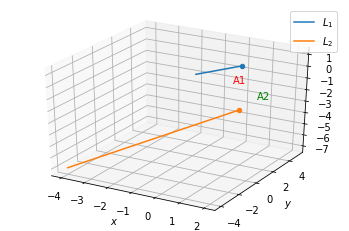
\includegraphics[width=\columnwidth]{solutions/su2021/2/32/download (7).png}
\caption{Skew Lines}
\label{linform/32/fig: Skew Lines}	
\end{figure}
